\documentclass[letterpaper,twocolumn,amsmath,amsfont,amssymb,english,aps,jcp,preprintnumbers,groupaddress,nofootinbib,tightenlines]{revtex4}

\usepackage{graphicx}


%\documentclass[aps,prb,letterpaper,twocolumn,nofootinbib,showkeys]{revtex4-1}
%\documentclass[aps,amssymb,prl,letterpaper,twocolumn,nofootinbib,showkeys]{revtex4-1}

%\usepackage[backend=bibtex]{biblatex}

%    backend=biber,
%    style=authoryear,
%    natbib=true,
%    sortlocale=en_US,
%    url=false,
%    doi=true,f
%    eprint=false
%]{biblatex}
%\usepackage{hyperref}


\newcommand{\mat}[1]{\boldsymbol{#1}}
\newcommand{\matT}[1]{\boldsymbol{#1}^\dagger}
\newcommand{\ot}{ {\scriptstyle \otimes}_{ \tau } }

%%\hypersetup{pdftitle={FreeON Project Report 1}}
%\hypersetup{pdfauthor={Matt Challacombe and Nicolas Bock}}
%\hypersetup{pdfsubject={A SpAMM Stabilized Newton Schulz Preconditioner: Fighting Error with Error}}

%\bibstyle{aipnum4-1}

\begin{document}

\title{On Stability of Newton Schulz Iterations in an Approximate Algebra}

\author{Matt Challacombe}
\email{matt.challacombe@freeon.org}
\homepage{http://www.freeon.org}
\affiliation{Theoretical Division, Los Alamos National Laboratory}

\author{Nicolas Bock}
\email{nicolasbock@freeon.org}
\homepage{http://www.freeon.org}
\affiliation{Theoretical Division, Los Alamos National Laboratory}

%\begin{abstract}
%Forward look
%\end{abstract}

\maketitle
\section{Introduction}

In many areas of application, finite correlations lead to matrices with decay properties.  By decay, we mean an approximate 
(perhaps bounded \cite{}) inverse relationship between matrix elements and an associated distance;  this may be a simple inverse 
exponential relationship between elements and the Cartesian distance between support functions, or it may 
involve a generalized distance, {\em e.g.}~ a statistical measure between strings.  
In electronic structure,  correlations manifest in decay properties of the gap shifted matrix 
sign function, as projector of the effective Hamiltonian (Fig.~\ref{figure1}).  
More broadly, matrix decay properties may coorespond to statistical matrices 
\cite{penrose1974,voit00,Anselin2003,Hardin2013,Krishtal2014}, including learned correlations in a 
generalized, non-orthogonal metric \cite{}. More broadly still, problems with local, non-orothogonal support 
are often solved with congruential transformations of the matrix inverse square root \cite{Lowdin56,naidu11} or a related factorization \cite{Krishtal2014};
these transformations correlate local support with a representation independent form, {\em eg.}~of the eigenproblem. 
Interestingly, the matrix sign function and the matrix inverse square root function are related by Higham's identity:
\begin{equation}
\rm{sign} \left( \begin{bmatrix} 0 & \mat{s}      \\ \mat{I}       & 0\end{bmatrix} \right)  =
                 \begin{bmatrix} 0 & \mat{s}^{1/2} \\ \mat{s}^{-1/2} & 0\end{bmatrix}  .
\end{equation}
A complete overivew of matrix function theory and computation is given in Higham's enjoyable reference \cite{Higham08}. 

A well conditioned matrix $\mat{s}$ may often correspond to matrix sign and inverse square root functions with rapid exponential decay, 
and be amenable to the sparse matrix approximation
$\bar{\mat{s}} = \mat{s}+ \mat{\epsilon}^{\mat{s}}_\tau$, where $\mat{\epsilon}^{\mat{s}}_\tau$ is the error introduced according to some  
criteria $\tau$.  Supporting this approximation are usefull bounds to matrix function elements \cite{Benzi99b, }.  
The criteria $\tau$ might be a drop-tolerence, 
$\epsilon^{\mat{s}}_{\tau} = \{-s_{ij}*\hat{\mat{e}}_i \, | \, |s_{ij}|<\tau \}$, a radial cutoff, 
$\epsilon^{\mat{s}}_{\tau} = \{-s_{ij}*\hat{\mat{e}}_i \, | \, \lVert \mat{r}_i - \mat{r}_j \rVert > \tau \}$, 
or some other approach to truncation, perhaps involving a sparsity pattern chosen {\em a priori}. 
Then, conventional computational kernels may be employed, such as the sparse general matrix-matrix multiply 
($\tt{SpGEMM}$) \cite{Gustavson78, Toledo97,challacombe00,bowler00}, yeiding fast solutions for multiplication rich iterations and a modulated fill in. 
These and related incomplete/inexact approaches to the computation of sparse approximate matrix functions often lead to ${\cal O}(n)$ 
algorithms, finding wide use in technologically important preconditioning schemes, the information sciences, electronic structure and many
other disciplines.  Comprehensive surveys of these methods in the numerical linear algebra are given by Benzi \cite{Benzi99,Benzi02}, and
by Bowler \cite{Bowler12} and Benzi \cite{Benzi13} for electronic structure.

\begin{figure}[t]\label{figure1}
 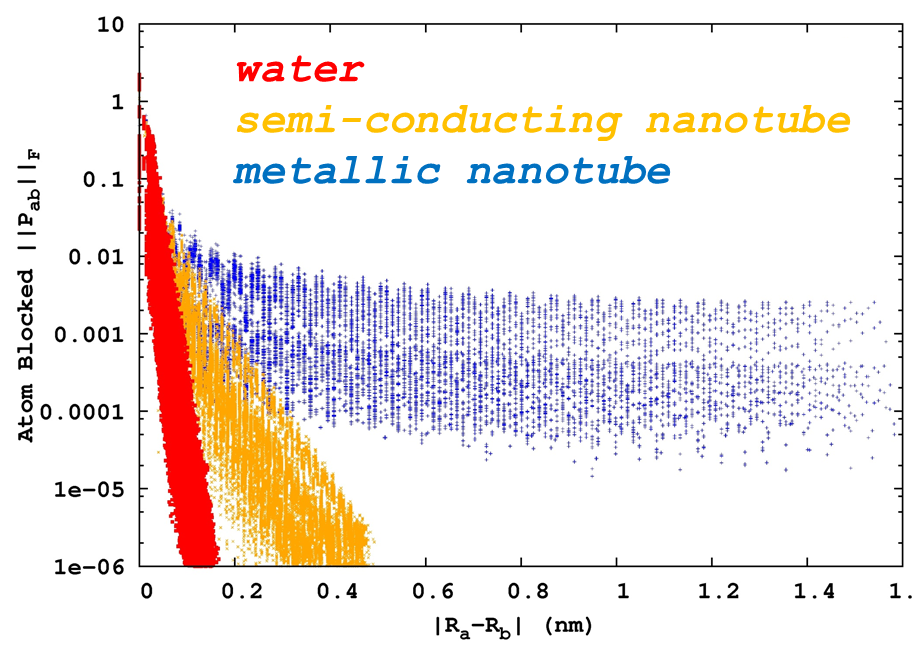
\includegraphics[width=3.5in]{decay_picture.png}
  \caption{Examples from electronic structure of decay for the spectral projector (gap shifted sign function) with respect to local (atomic) support.  
           Shown is decay for systems with correlations that are short (insulating water), medium (semi-conducting 4,3 nanotube), and 
           long (metalic 3,3 nanotube) ranged,  from exponential (insulating) to algebraic (metallic). }
\end{figure}

Because the truncated multiplication is controled only by absolute, addititve errors in the  product,   
\begin{equation}
\overline{ \mat{a} \cdot \mat{b} }\; = \; \mat{a}\cdot\mat{b} \; +\; \mat{\epsilon}^{\mat{a}}_\tau \cdot \mat{b} \;+\;
 \mat{a} \cdot \mat{\epsilon}^{\mat{b}}_\tau  \; + \;   {\mathcal O}(\tau^2)
\end{equation}
achieving sparse, stable and rapidly convergent iteration for ill-conditioned problems can be challenging \cite{}.  In cases of 
extreme degeneracy,  hierarchical semi-seperable (reduced rank) algorithms  can offer effective complexity reduction \cite{}.
However, many pratical cases are somewhere in-between sparse and meaningfully degenerate regimes; effectively dense but without
an exploitable reduction in rank.  This is the case in electronic structure for strong but non-metalic correlation, 
{\em e.g.}~towards the Mott transition \cite{}, and also in the case of local atomic support towards completeness \cite{Others, Hutter, Gigi}. 

\pagebreak
In this contribution, we consider an $N$-body approach to the approximation of matrix functions with decay, 
based on the quadtree data structure \cite{wise, samet} 
\begin{equation}
\mat{a}^i = \begin{bmatrix} \,  \mat{a}^{i+1}_{00} \, & \,  \mat{a}^{i+1}_{01} \,  \\[0.2cm]  \, \mat{a}^{i+1}_{10} \,  & \,\mat{a}^{i+1}_{11} \, \end{bmatrix} \, ,
\end{equation}
and orderings that are locality preserving \cite{}.  Orderings that preserve data locality are well developed in the
database theory \cite{}, providing fast spatial and metric querries.  
Locality enabled, fast data access is central to the $N$-Body approximation \cite{}, and an important problem 
for enterprise \cite{} and runtime systems \cite{}, with memory hierarchies becoming increasingly assynchronous and decentralized \cite{cache}.  
For matrices with decay, orderings that preserve locality lead to block-by-magnitude matrix structures with well 
segregated neighborhoods, inhabited by matrix elements of like size, and efficiently resolved by the quadtree data structure \cite{}.

With block-by-magnitude ordering of matrices $\mat{a}$ and $\mat{b}$, 
the Sparse Approximate Matrix Multiplication ($\tt SpAMM$) kernel,  $\ot$, carries out fast 
occlusion culling of insignifcant volumes in the product octree:
\begin{widetext}
\begin{equation}
\mat{a}^{i} \ot \mat{b}^{i} = 
\left\{
        \begin{array}{ll}
                 \emptyset \quad \tt{if}\quad \lVert \mat{a}^i \rVert \lVert \mat{b}^i \rVert < \tau \\[0.2cm]
                 \mat{a} ^i \cdot \mat{b}^i \quad  \tt{if}(i=\tt{leaf}) \\[0.2cm]
\begin{bmatrix} \mat{a}^{i+1}_{00} \ot \mat{b}^{i+1}_{00} +\mat{a}^{i+1}_{01} \ot \mat{b}^{i+1}_{10} \; , \; &
                \mat{a}^{i+1}_{00} \ot \mat{b}^{i+1}_{01} +\mat{a}^{i+1}_{01} \ot \mat{b}^{i+1}_{11}  \\[0.2cm] 
                \mat{a}^{i+1}_{00} \ot \mat{b}^{i+1}_{01} +\mat{a}^{i+1}_{01} \ot \mat{b}^{i+1}_{11} \; , \; & 
                \mat{a}^{i+1}_{00} \ot \mat{b}^{i+1}_{01} +\mat{a}^{i+1}_{01} \ot \mat{b}^{i+1}_{11}   
\end{bmatrix}  \quad \tt{else}
                \end{array}
              \right.  \, ,
\end{equation}
\end{widetext}
with errors bounded by sub-multiplicative norms, $\lVert \cdot \rVert \equiv \lVert \cdot \rVert_F$, and the Cauchy-Schwarz inequality \cite{kahan}.
$\tt SpAMM$ is similar in spirit to compressed sensing kernels for sketching the matrix product \cite{Kutzkov2012, Pagh2013}.  However, 
instead of using the FFT to compute the sketch, compression is achieved simply through fast querry of the product decay.

The $\tt SpAMM$ kernel stands in contrast to methods based on random matrix theory, which enhance matrix conditioning via 
homogenization \cite{pan, DiahLi and Parket Scott}, and also with distributed memory implementations of the $\tt SpGEMM$, which 
enjoy work load homogenisation through radomization \cite{}.  Differences between the $\tt SpAMM$ kernel and randomized 
approaches to the $\tt SpGEMM$ are reviewed in Ref.[\cite{}], and with the $\tt GEMM$ in Ref.\cite{}.

The total error associated with $\ot$ is 
\begin{equation}
\mat{\Delta}^{a\cdot b}_{\tau}=\mat{a} \ot \mat{b}-\mat{a}\cdot \mat{b} \, ,
\end{equation}
corresponding to the occluded contraction volume, and obeys the multiplicative bound 
\begin{equation}
\lVert \mat{\Delta}^{a \cdot b}_{\tau} \rVert \, \leq \, \tau \, \lVert \mat{a} \rVert  \,  \lVert \mat{b} \rVert \, ,
\end{equation}
which is {\em stabile} \cite{DemmelnHolz2007} and offering the potential for {\em relative} error control.
Unlike roundoff error however, the $\tt SpAMM$ error is deterministic,
leading to a non-associative algebra and the development of error flows associated with the Lie bracket
\begin{equation}
\left[ \mat{a} , \mat{b} \right]_{\tau} = \mat{a} \ot \mat{b}-\mat{b} \ot \mat{a}  
=  \left[ \mat{a} , \mat{b} \right]
+ \mat{\Delta}^{a\cdot b}_{\tau} -\mat{\Delta}^{b\cdot a}_{\tau} \,.
\end{equation}
While the $\tt SpAMM$ occlusion criteria is deterministic, Eq.~(\ref{spamm}), 
there may be alternative criteria for occlusion and related approximations that 
achieve simililar accuracies at lower cost, or that achieve supperior error control under iteration, 
perhaps involving persistence (learning) and/or probabilistic sampling \cite{Drineas}.  

\section{First Order Newton-Shulz Iteration}

The approximation of the matrix sign and inverse square root via first order Newton Schulz (NS) iteration 
has a number of attractive features, notably multiplication richness and quadratic convergence in the basin of convergence. 
Developed extensively by Higham \cite{}, NS  yeilds resolution of the identity through the square root and its inverse \cite{}:
\begin{equation}
sign \left( \mat{s} \right) =\mat{s}^{1/2} \cdot \mat{s^{-1/2}} \, .
\end{equation}
For well conditioned problems, incomplete/inexact approximations and the $\tt SpGEMM$ kernel offer fast solutions \cite{}.
For ill-conditioned problems however, fill in remains a challenge \cite{}, showing up well before matrix-compression 
technologies become effective.   

In this contribution, we develop the $\tt SpAMM$ kernel for NS iteration at index $k$, focusing on eigenvector (basis) fidelity to the
positive definate argument $\mat{s}$, and stability as the residual $\mat{x}_k $ tends towards 
idempotence, $\mat{x}_k \rightarrow {sign}\left( \mat{s} \right) $, with 
 $\mat{y}_k \rightarrow \mat{s}^{1/2}$  and $\mat{z}_k \rightarrow \mat{s}^{-1/2}$ \cite{higham}.  first order map, scaling and so on
In the first order $m$ .  Scaling developed by Jie and co.
There are several NS forms that are in principle equivalent, but which behave very 
differently for ill-conditioned problems. 

In our notation these iterations naive: 
\begin{eqnarray}
\mat{z}^{\tt naiv}_{k}  &\leftarrow& \mat{z}_{k-1}  \cdot m \left( \mat{x}_{k-1} \right) \\
\mat{x}^{\tt naiv}_{k} &\leftarrow& \mat{z}_{k} \cdot \mat{s} \cdot \mat{z}_{k}
\end{eqnarray}


We begin our development with 
the analysis of Bai and Demmel \cite{}, Byers, He and Mehrmann \cite{} and Higham, Ref.\cite{} Section 5.7.
These authors show that, once convergence has been achieved, than any (initial) error $\delta \mat{s}$ about
$\mat{s}$ is quenched 


% has the property $sign \left(  \mat{s}^* + \delta \mat{s) } = 


% variation of $sign$ about an idempotent fixed point $\mat{s}^*$ with an initial 
% commuting error 
% $\delta \mat{s}$ has the property $sign \left(  \mat{s}^* + \delta \mat{s) } = 
% sign \left(  \mat{s}^* \right) $.  



\subsubsection{The Scaled Map}


In addition to retaining the basis with each step $k$ 
\footnote{Sometimes refered to as a ``variational'' property, associated with retaining the basis through gradient 
terms, in early work on $\cal$ approximation of the spectral projector through optimization \cite{}.}, 
NS allows to re-introduce the eigenvectors at any 
level of $\tt SpAMM$ precision, {\em e.g.}~after the basin of convergence has been reached.   
The ability to retain the basis in functional approximation is a key feature of the NS method, in 
contrast to the exponential error growth that develops in nested polynomial approximation \cite{},
a limiting issue in many applications \cite{}.  Instead, NS allows correction of a converged residual 
at previous $\tt SpAMM$ resolutions with little additional cost \cite{}, {\em e.g.} 
\begin{equation}  
\mat{s}^{-1/2} \approx \mat{z}^{\tau_m} \; {\scriptstyle \otimes}_{\tau_m} \; \mat{z}^{\tau_{m-1}}{\scriptstyle \otimes_{\tau_{m-1}}}
\; \ldots \; {\scriptstyle \otimes}_{\tau_{\scriptscriptstyle 0}} \; \mat{z}^{\tau_{\scriptscriptstyle 0}} \, ,
\end{equation}
with $\tau_m \; < \;  \tau_{m-1} \; < \; \ldots  \; < \; \tau_0$.  Efficiency is then determined by stability of the 
most extreme permisive preconditioning provided by $\mat{z}^{\tau_{\scriptscriptstyle 0}}$.

\section{Occlusion Flows}

$\delta \mat{x}_k$ and $\delta \mat{z}_k$ arrize from itteration with $\ot$, and are deterministic 
flows away from the manifold of $\mat{s}$ determined by sensitivity of the NS iteration to these 
numerical insults. 


\begin{equation}
\delta \mat{x}^{\rm{naiv}}_k =   \delta  \widetilde{ \mat{z}}_{k} \cdot \mat{s} \cdot \widetilde{\mat{z}}_{k} 
                           +  \widetilde{\mat{z}}_{k} \cdot \mat{s} \cdot \! \delta \widetilde{\mat{z}}_{k} 
\end{equation}



\begin{equation}
\delta \mat{x}^{\rm{dual}}_k =   \delta  \widetilde{ \mat{y}}_{k} \cdot \widehat{\mat{z}}_{k} 
                           +  \widetilde{\mat{y}}_{k} \cdot \delta \widetilde{\mat{z}}_{k} 
\end{equation}


\begin{eqnarray}
\widetilde{\mat{x}}_k &=& f \left[\widetilde{\mat{z}}_{k-1} , \widetilde{\mat{x}}_{k-1} \right] \\ 
&=&
\tt{m} \left[ \widetilde{\mat{x}}_{k-1}\right] \cdot \widetilde{\mat{z}}^\dagger_{k-1}  
\cdot \mat{s} \cdot \widetilde{\mat{z}}_{k-1} \cdot \tt{m}\left[ \widetilde{\mat{x}}_{k-1} \right] 
\nonumber
\end{eqnarray}

\begin{equation}
\delta \mat{x}_k = {f}_{\delta \mat{z}_{k-1}}  \, \lVert \delta \mat{z}_{k-1} \rVert 
                              +  {f}_{\delta \mat{x}_{k-1}}   \, \lVert \delta \mat{x}_{k-1} \rVert 
                                                                                      + {\cal{O}} \left(  \tau^2 \right)
\end{equation}

generalized Gateaux differential

\begin{eqnarray}
f_{\delta \mat{z}_{k-1}} &=& \lim_{\tau \rightarrow 0} \frac{ f [ \mat{z}_{k-1} +\tau  \delta \widehat{\mat{z}}_{k-1}, \widetilde{\mat{x}}_{k-1} ]
-f [\, \mat{z}_{k-1}, \widetilde{\mat{x}}_{k-1} ]  }{\tau} \nonumber  \\[0.1cm] 
&=&{L}_{\widetilde{\mat{x}}_k}\left(\widetilde{\mat{z}}_{k} , \delta \widehat{\mat{z}}_{k-1} \right)  
\end{eqnarray}

\begin{eqnarray}
f_{\delta \mat{x}_{k-1}} &=& \lim_{\tau \rightarrow 0} \frac{ f [ \widetilde{\mat{z}}_{k-1}, \mat{x}_{k-1} + \tau \delta \widehat{\mat{x}}_{k-1} ]
-f [ \widetilde{\mat{z}}_{k-1}, \mat{x}_{k-1} ]  }{\tau} \nonumber  \\[0.1cm] 
&=&{L}_{\widetilde{\mat{x}}_k}\left(\widetilde{\mat{z}}_{k} , \delta \widehat{\mat{x}}_{k-1} \right)  
\end{eqnarray}

\begin{multline}
{L}_{\widetilde{\mat{x}}_k}\left(\widetilde{\mat{z}}_{k} , \delta \widehat{\mat{x}}_{k-1} \right) 
= \delta \widehat{\mat{x}}^\dagger_{k-1} \cdot   \tt{m}'\left[\mat{x}_{k-1} \right] \cdot 
\{\widetilde{\mat{z}}^\dagger_{k-1}  \cdot \mat{s} \cdot \widetilde{\mat{z}}_{k} \}  \\
+ \{ \widetilde{\mat{z}}^\dagger_{k} \cdot \mat{s} \cdot  \widetilde{\mat{z}}_{k-1} \} 
\cdot \tt{m}'\left[\mat{x}_{k-1} \right]  \cdot \delta \widehat{\mat{x}}_{k-1} 
\end{multline}

\begin{multline}
{L}_{\widetilde{\mat{x}}_k}\left(\widetilde{\mat{z}}_{k} , \delta \widehat{\mat{z}}_{k-1} \right) = 
\{ \tt{m}\left[\mat{x}_{k-1} \right]  \cdot \delta {\widehat{\mat{z}}}^\dagger_{k-1} 
 \cdot \mat{s} \} \cdot \widetilde{\mat{z}}_{k} \\
+\widetilde{\mat{z}}^\dagger_{k} \cdot \{ \mat{s} \cdot \delta {\widehat{\mat{z}}}_{k-1}
\cdot \tt{m}\left[\mat{x}_{k-1} \right]    \} 
\end{multline}

\begin{equation}
 \{ \widetilde{\mat{z}}^\dagger_{k} \cdot \mat{s} \cdot  \widetilde{\mat{z}}_{k-1} \} 
\rightarrow \mat{p}_+\left[\mat{s} \right]
\end{equation}

\begin{equation}
\{ \mat{s} \cdot \delta {\widehat{\mat{z}}}_{k-1}
\cdot \tt{m}\left[\mat{x}_{k-1} \right]    \} 
\rightarrow \mat{n}\left[\mat{s} \right]
\end{equation}

\section{Implementation}

\subsection{Methods}
FP, F08, OpenMP 4.0

\subsection{A Modified NS Map}

\subsection{$\delta \mat{x}_k$ and $\delta \mat{x}_k$ channels}
tau= Figure showing channels etc.  

\subsection{Convergence}
Map switching and etc based on TrX


\section{Ill-Conditioned Support}

\subsection{ 3,3 carbon nanotube with diffuse $sp$-function}
double exponential (Fig.)

\subsection{Water with triple zeta and double polarization}
Here's looking at you Jurg...

\section{Experiments}

\subsection{Occlusion Error Flows}
\begin{figure}[h]
  \caption{equation...}
 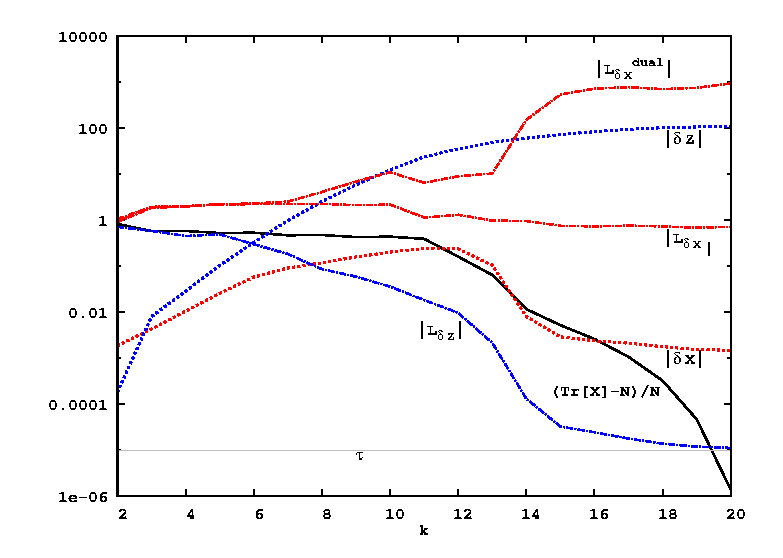
\includegraphics[width=3.5in]{8x_33_nanotube_cond10_tau-5.eps}
 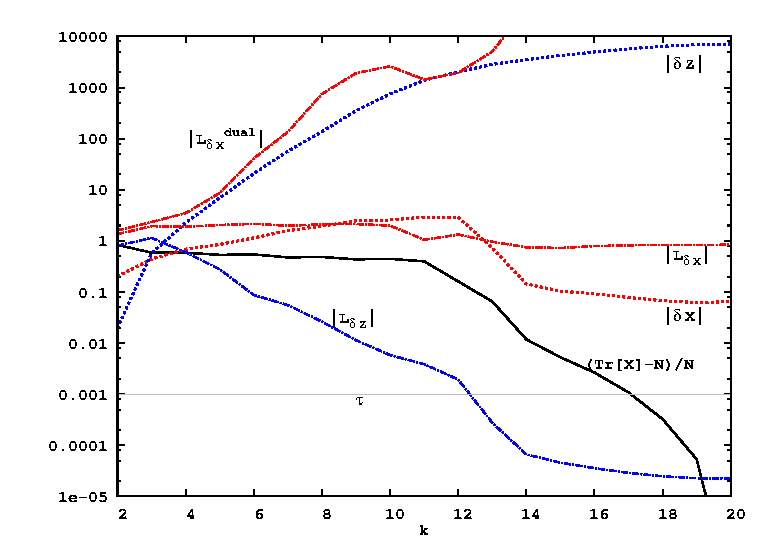
\includegraphics[width=3.5in]{8x_33_nanotube_cond10_tau-3.eps}
\end{figure}
\begin{figure}[h]
  \caption{equation...}
 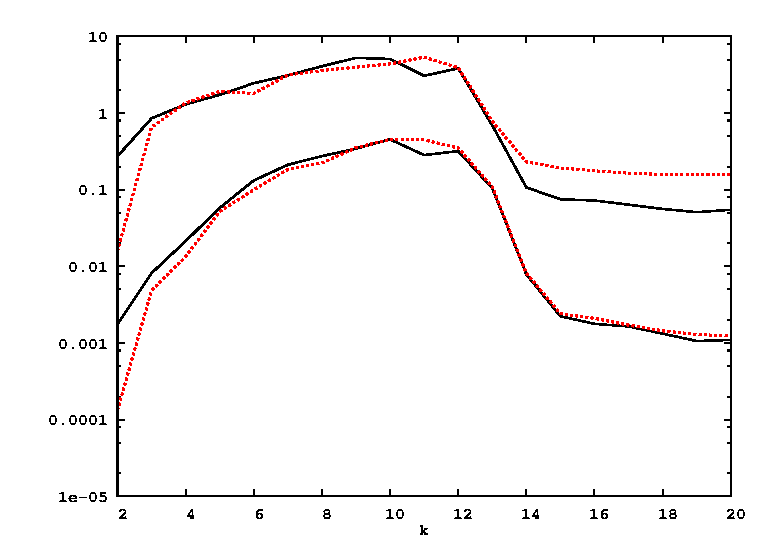
\includegraphics[width=3.5in]{8x_33_nanotube_cond10_compare_errors.eps}
\end{figure}

\subsection{Comments}

\begin{multline}
 \delta {\mat{z}}_{k-1} \approx \Delta^{\widetilde{\mat{z}}_{k-2} \cdot \tt{m}\left[ \widetilde{\mat{x}}_{k-2}\right]}_\tau 
+ \mat{z}_{k-2} \cdot \tt{m}'\left[ \widetilde{\mat{x}}_{k-2}\right] \cdot \delta \mat{x}_{k-2} \\
+\delta \mat{z}_{k-2} \cdot \tt{m} \left[\widetilde{\mat{x}}_{k-2} \right] 
\end{multline}

\begin{multline}
\lVert \delta {\mat{z}}_{k-1} \rVert \lesssim
\lVert \mat{z}_{k-2} \rVert \left( \;  \tau \, \lVert \tt{m} \left[\widetilde{\mat{x}}_{k-2} \right]  \rVert \right.   \\ \left.
+ \; \lVert \delta {\mat{x}}_{k-2} \rVert   \lVert \tt{m}' \left[\widetilde{\mat{x}}_{k-2} \right] \rVert \; \right)
\end{multline}

\begin{equation}
\lVert \mat{z}_{k} \rVert  \rightarrow \sqrt{\kappa\left(\mat{s} \right)}
\end{equation}

\subsection{Querry Surfaces}

\begin{figure}[h]
  \caption{equation...}
\fbox{ 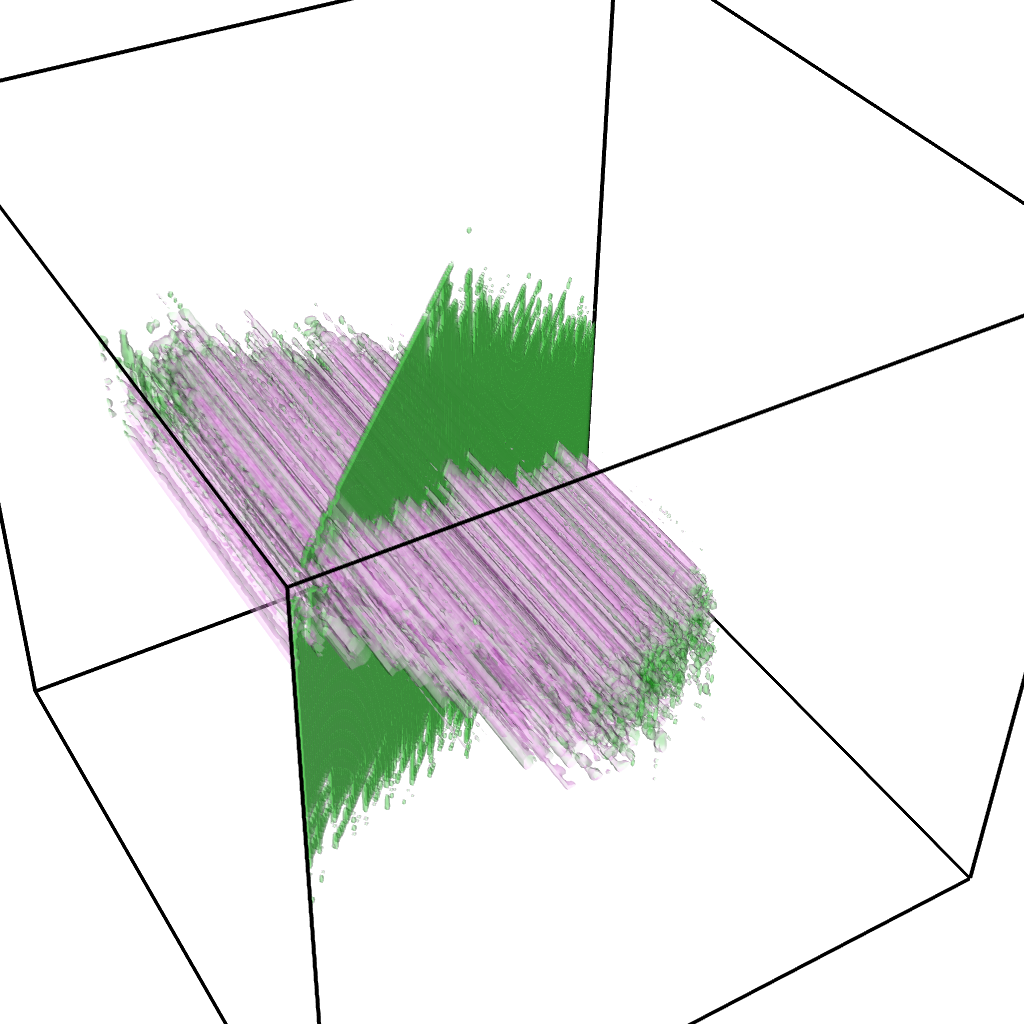
\includegraphics[width=1.5in,trim={6cm 6cm 6cm 6cm},clip]{y_15_tube_5_36.png}} 
\fbox{ 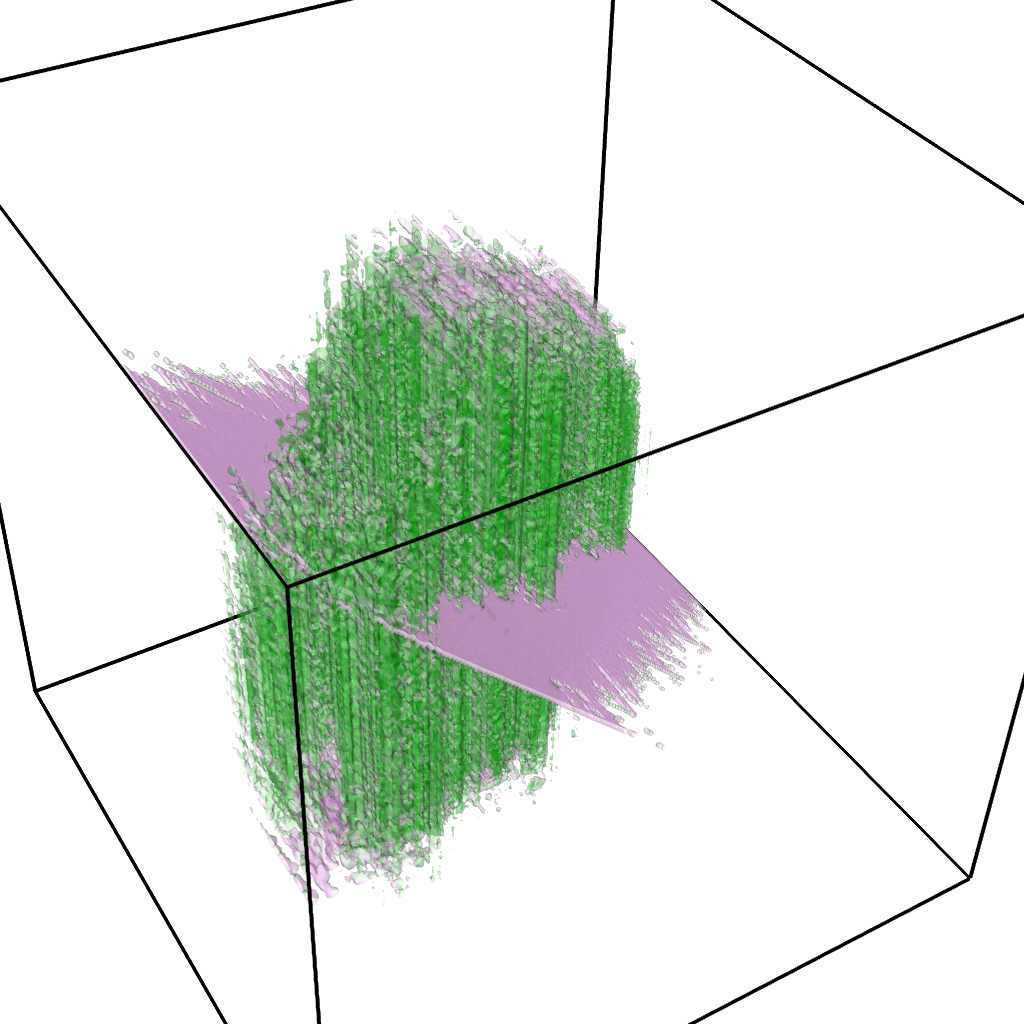
\includegraphics[width=1.5in,trim={6cm 6cm 6cm 6cm},clip]{z_15_tube_5_36.png}}
\end{figure}


\begin{figure}[h]
  \caption{equation...}
\fbox{ 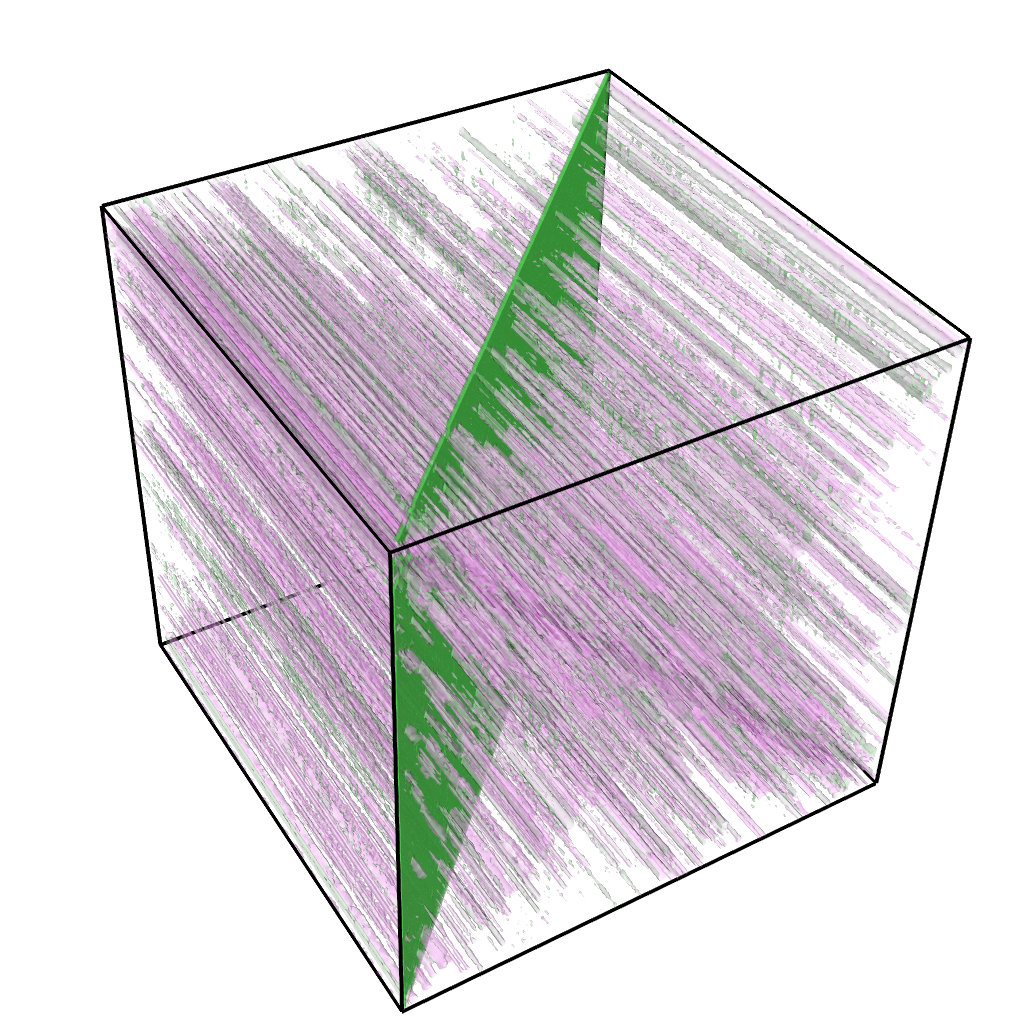
\includegraphics[width=1.5in,trim={6cm 6cm 6cm 6cm},clip]{y_15_water.png}} 
\fbox{ 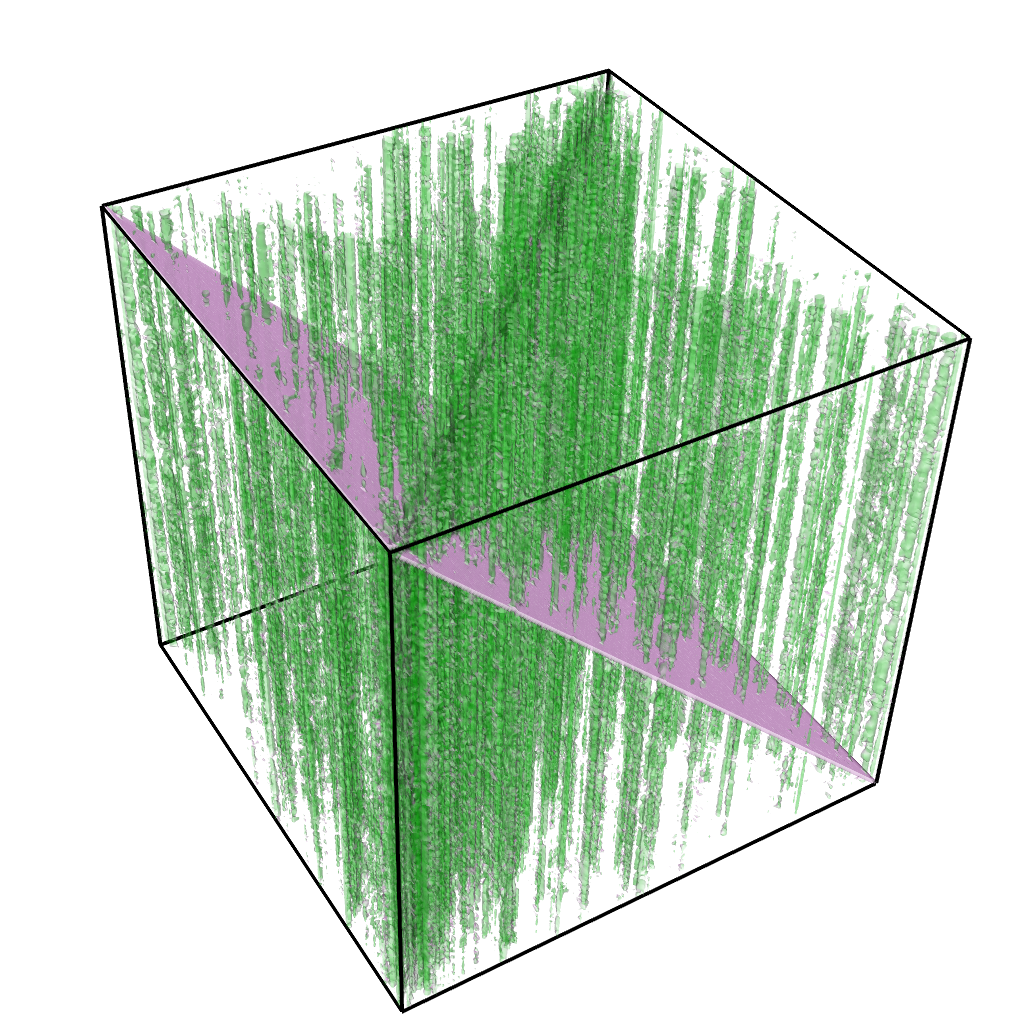
\includegraphics[width=1.5in,trim={6cm 6cm 6cm 6cm},clip]{z_15_water.png}}
\end{figure}


\subsection{Comments}

\subsection{Found Contraction}

\subsection{Comments}
Pictures of the spamm structure

\section{Conclusion}

%%eg vs row-col picture.  Example of exact exchange w/DBSR 

\bibliography{MatrixFunctions}

\end{document}
